%##noBuild
\newpage
\section{Widoki}

\subsection{WYCIECZKI OSOBY}
\begin{verbatim}
CREATE VIEW WYCIECZKI_OSOBY AS
  SELECT A.KRAJ, A.DATA, A.NAZWA, C.IMIE, C.NAZWISKO, B.STATUS
  FROM WYCIECZKI A
         INNER JOIN REZERWACJE B ON A.ID_WYCIECZKI = B.ID_WYCIECZKI
         INNER JOIN OSOBY C ON B.ID_OSOBY = C.ID_OSOBY
\end{verbatim}

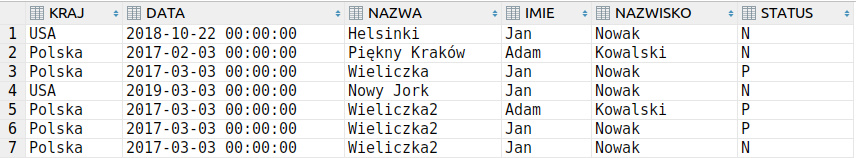
\includegraphics[width=\linewidth]{./images/wycieczki_osoby.png}

\subsection{WYCIECZKI OSOBY POTWIERDZONE}
\begin{verbatim}
CREATE VIEW WYCIECZKI_OSOBY_POTWIERDZONE AS
  SELECT W.KRAJ, W.DATA, W.NAZWA, O.IMIE, O.NAZWISKO, R.STATUS
  FROM WYCIECZKI W 
         INNER JOIN REZERWACJE R ON W.ID_WYCIECZKI = R.ID_WYCIECZKI
         INNER JOIN OSOBY O ON R.ID_OSOBY = O.ID_OSOBY
  WHERE R.STATUS = 'P'
\end{verbatim}

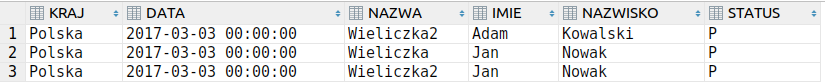
\includegraphics[width=\linewidth]{./images/wycieczki_osoby_potwierdzone.png}

\subsection{WYCIECZKI PRZYSZLE}
\begin{verbatim}
CREATE VIEW WYCIECZKI_PRZYSZLE AS
  SELECT W.KRAJ, W.DATA, W.NAZWA, O.IMIE, O.NAZWISKO, R.STATUS
  FROM WYCIECZKI W
         INNER JOIN REZERWACJE R ON W.ID_WYCIECZKI = R.ID_WYCIECZKI
         INNER JOIN OSOBY O ON R.ID_OSOBY = O.ID_OSOBY
  WHERE W.DATA > (SELECT CURRENT_DATE FROM DUAL)
\end{verbatim}

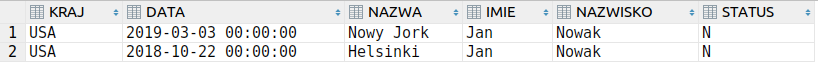
\includegraphics[width=\linewidth]{./images/wycieczki_przyszle.png}

\subsection{WYCIECZKI MIEJSCA}
\begin{verbatim}
CREATE VIEW WYCIECZKI_MIEJSCA AS
  SELECT W.KRAJ,
         W.DATA,
         W.NAZWA,
         W.LICZBA_MIEJSC,
         W.LICZBA_MIEJSC -
         NVL((SELECT COUNT(*) FROM REZERWACJE R WHERE W.ID_WYCIECZKI = R.ID_WYCIECZKI GROUP BY R.ID_WYCIECZKI),
             0) AS LICZBA_MIEJSC_WOLNYCH
  FROM WYCIECZKI W
\end{verbatim}

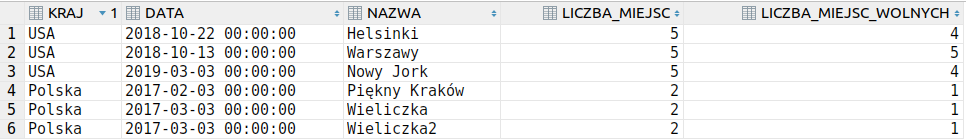
\includegraphics[width=\linewidth]{./images/wycieczki_miejsca.png}

\subsection{DOSTĘPNE WYCIEZKI}
\begin{verbatim}
CREATE VIEW DOSTĘPNE_WYCIEZKI AS
  SELECT W.KRAJ,
         W.DATA,
         W.NAZWA,
         W.LICZBA_MIEJSC,
         W.LICZBA_MIEJSC -
         NVL((SELECT COUNT(*) FROM REZERWACJE R 
         WHERE W.ID_WYCIECZKI = R.ID_WYCIECZKI GROUP BY R.ID_WYCIECZKI),
             0) AS LICZBA_MIEJSC_WOLNYCH
  FROM WYCIECZKI W
  WHERE W.LICZBA_MIEJSC -
        NVL((SELECT COUNT(*) FROM REZERWACJE R WHERE W.ID_WYCIECZKI = R.ID_WYCIECZKI GROUP BY R.ID_WYCIECZKI),
            0) > 0
    AND (SELECT CURRENT_DATE FROM DUAL) < W.DATA
\end{verbatim}

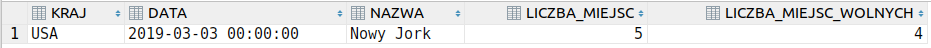
\includegraphics[width=\linewidth]{./images/dostepne_wycieczki.png}

\subsection{REZERWACJE DO ANULOWANIA}
\begin{verbatim}
CREATE VIEW REZERWACJE_DO_ANULOWANIA AS
  SELECT R.NR_REZERWACJI AS NR_REZERWACJI_DO_ANULOWANIA
  FROM REZERWACJE R
         INNER JOIN WYCIECZKI W ON W.ID_WYCIECZKI = R.ID_WYCIECZKI
  WHERE R.STATUS = 'N'
    AND W.DATA - (SELECT CURRENT_DATE FROM DUAL) < 7
    AND W.DATA > (SELECT CURRENT_DATE FROM DUAL)
\end{verbatim}

\begin{minipage}{0.40\textwidth}
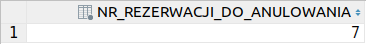
\includegraphics[width=\linewidth]{./images/rezerwacje_do_anulowania.png}
\end{minipage}